\documentclass[12pt]{article}

\usepackage{amsmath}
\usepackage{amssymb}
\usepackage{amsfonts}
\usepackage{polski}
\usepackage{verbatim}
\usepackage[utf8]{inputenc}
\usepackage[polish]{babel}
\usepackage[T1]{fontenc}
\usepackage{graphicx}
\usepackage{caption}
\usepackage{enumitem}
\usepackage{hyperref}
\usepackage{natbib}
\usepackage{graphicx}
\usepackage{datetime}
\usepackage{multirow}
\usepackage{array}
\newdateformat{mydate}{\twodigit{\THEDAY}.\twodigit{\THEMONTH}.\THEYEAR r.}
\usepackage{enumitem}
\usepackage{footnote}
\setlist{
	noitemsep,
	listparindent=\parindent,
	parsep=0pt,
}
\makesavenoteenv{tabular}
\makesavenoteenv{table}

\usepackage{xparse}

\textheight 23.2 cm
\textwidth 6.0 in
\hoffset = -0.5 in
\voffset = -2.4 cm

\begin{document}

\begin{titlepage}
	\begin{flushright}
		{\mydate\today}\\
	\end{flushright}
	\vskip30ex

	\begin{center}
		\Large {\bf{
				System do zdalnej pracy w środowisku graficznym wykorzystujący maszyny wirtualne QEMU z akceleracja sprzętową\\
			}}
		\vskip2ex
		\bf{Sprawozdanie z testów\\}
		\vskip2ex
		\small { Autorzy: Krzysztof Smogór, Piotr Widomski\\  }
		\small { Promotor: Dr inż. Marek Kozłowski\\ }
	\end{center}
\end{titlepage}

\tableofcontents

\newpage

\section{Testy jednostkowe}

\subsection{Testy jednostkowe frontendu}

Do testowania aplikacji klienckiej oraz panelu administratora wykorzystaliśmy testy jednostkowe. Testowane były zarówno serwisy, jak i komponenty odpowiadające za widoki. Dzięki testowaniu komponentów w zakresie DOMa uzyskaliśmy testowanie UI, które dopełnione zostało testami E2E.

\begin{figure}[!h]
	\centering
	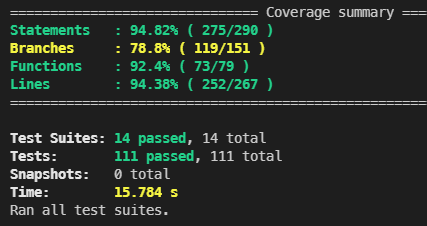
\includegraphics[width=0.7\linewidth]{res/client-test}
	\caption{Podsumowanie testów jednostkowych aplikacji klienckiej}
	\label{fig:client-test}
\end{figure}

\subsection{Biblioteka modelu systemu}

Klasy implementujące model systemu wydzielone zostały do osobnej biblioteki, która importowana jest do modułów jako pakiet nuget. Biblioteka ta zawiera proste klasy, służące do przechowywania informacji o stanie systemu. Do przetestowania jej użyliśmy testów jednostkowych, które badają poprawność działania funkcji udostępnianych przez klasy.

\subsection{Moduł nadzorcy oraz serwera wirtualizacji}

Moduły te są głównymi elementami systemu. Testowanie ich zostanie przeprowadzone za pomocą testów jednostkowych. Testowane będą wszystkie serwisy, z zastosowaniem mocków.

\section{Testy integracyjne}

\subsection {Testy integracji z libvirtem oraz vagrantem}

Przy integracji systemu z libvirtem oraz vagrantem musielismy sprawdzic następujące funkcjonalności:
\begin{enumerate}
	\item Włączanie maszyn poprzez vagranta
	\item Wyłączanie maszyn poprzez vagranta
	\item Sprawdzanie czy maszyna jest uruchomiona poprzez libvirta
	\item Pobranie adresu IP uruchomionej maszyny wirtualnej
\end{enumerate}

Aby testy miały sens potrzebowaliśmy konfiguracji XML do tworzenia maszyn \textit{transient} oraz gotowego lekkiego vagrant-boxa przy tworzeniu maszyn \textit{persistence}.
Przy testach libvirta wykorzystaliśmy obraz live ArchLinuxa, którego uruchamiamy w minimalnie przygotowanej konfiguracji.
Do testów vagranta skorzystaliśmy z lekkiego obrazu "generic/alpine38".
Przy testach konfiguracji sieciowej utworzyliśmy bridge sieciowy, który jest uwzględniony w konfiguracji uruchamianych maszyn wirtualnych.

Aby upewnić się, że wszystko działa prawidłowo skorzystaliśmy z mechaniki testów jednostkowych NUnit przy jednocześnie uruchomionym daemonie libvirta.

\begin{figure}[!h]
	\centering
	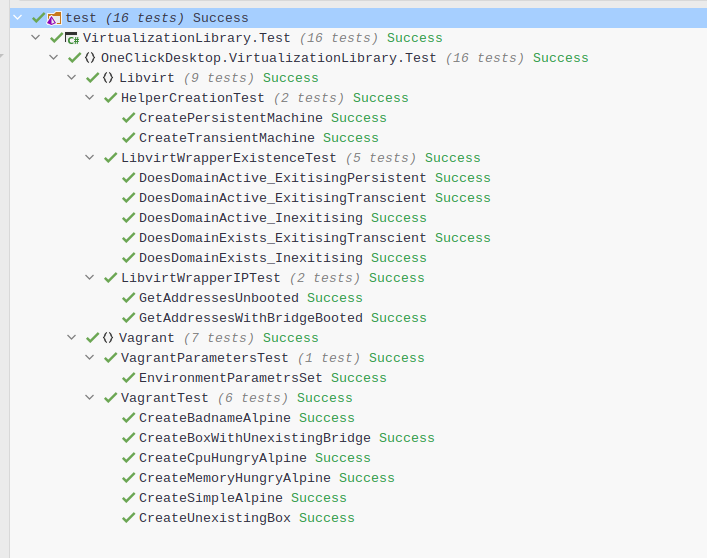
\includegraphics[width=0.7\linewidth]{res/virtsrvlib-test}
	\caption{Lista testów sprawdzających integrację z libvirtem i vagrantem}
	\label{fig:virtsrvlib-test}
\end{figure}

\subsection{Testy integracyjne z RabbitMQ}
Podczas tworzenia projektu wydzieliliśmy osobny moduł, którego celem jest obłożenie biblioteki API RabbitMQ w interfejs, który umożliwi wygodne użytkowanie brokera z poziomu głównych modułów systemu. Jako iż biblioteka ta nie posiada wewnętrznej logiki, a jedynie wywołuje odpowiednie funkcje brokera wiadomości, przetestowana została z użyciem testów integracyjnych. Testowana funkcjonalność obejmowała:
\begin{enumerate}
	\item Tworzenie punktów wymiany (exchange)
	\item Tworzenie kolejek i podłączanie ich do punktów wymiany
	\item Wysyłanie i odbieranie wiadomości (wraz z zaimplementowanym mechanizmem deserializacji)
	\item Wysyłanie wiadomości do konkretnych odbiorców
	\item Wykrywanie braku odbiorców
\end{enumerate}

W tym celu wykorzystaliśmy metodę analogiczną do testów z libvirtem, czyli mechaniki testów jednostkowych NUnit przy jednocześnie uruchomionym brokerze RabbitMQ.

\subsection {Wymierne efekty testów}
W wypadku testów integracyjnych zauważyliśmy wymierne efekty w czasie integracji.
Przy integrowaniu modułów nadzorcy i serwera wirtualizacji komunikacja i zarządzanie maszynami wirtualnymi zaczęło działać praktycznie przy pierwszym uruchomieniu.

\section{Testy E2E}
Aplikacja kliencka oraz panel administratora posiadają proste testy E2E, z wykorzystaniem platformy Cypress, spełniające równocześnie po części rolę testów UI. Testy te skupiają się na pojedynczych ekranach aplikacji oraz jej działaniu z perspektywy użytkownika.

Planujemy dodanie testów E2E realizujących wielokrokowe scenariusze testowe, zaczynające się od zalogowania do aplikacji.

\section{Scenariusze akceptacyjne}
Planujemy wykonać następujące testy akceptacyjne:

\subsection {Serwer wirtualizacji wyłącza się przy braku komunikacji z jakimkolwiek nadzorcą}
Przy starcie samodzielnego serwera wirtualizacji i wykryciu braku komunikacji z jakimkolwiek nadzorcą (poprzez brokera wiadomości) serwer powinien się wyłączyć z błędem.

Kroki:
\begin{enumerate}
	\item Włącz serwer wirtualizacji.
	\item Wyświetl błąd i zakończ działanie.
\end{enumerate}

\subsection {Serwer wirtualizacji wyłącza się przy utracie komunikacji z nadzorcami}
Po poprawnym starcie systemu z 1 nadzorca oraz 1 serwerem wirtualizacji serwer powinien wyłączyć się po wyłączeniu się ostatniego nadzorcy.

Kroki:
\begin{enumerate}
	\item Włącz brokera wiadomości wewnętrznego oraz zewnętrznego.
	\item Włącz aplikację nadzorcy.
	\item Włącz aplikację serwera wirtualizacji.
	\item Poczekaj na prawidłowy start systemu.
	\item Wyłącz nadzorcę lub brokery wiadomości.
	\item Poczekaj na wykrycie braku nadzorców (brak otrzymanych wiadomości)
	\item Wyświetl błąd i zakończ działanie.
\end{enumerate}

\subsection{Typowe użycie systemu przez użytkownika}
Użytkownik podłącza się do systemu składającego się z 1 nadzorcy oraz 1 serwera wirtualizacji, gdzie działa przynajmniej jedna wolna maszyna.
Powinien prawidłowo otrzymać sesje oraz po odłączeniu się maszyna powinna zostać wyłączona po 15 minutach(czas konfigurowalny)

Kroki:
\begin{enumerate}
	\item Włącz brokera wiadomości wewnętrznego oraz zewnętrznego.
	\item Włącz aplikację nadzorcy.
	\item Włącz aplikację serwera wirtualizacji.
	\item Poczekaj na uruchomienie przynajmniej jednej maszyny wirtualnej.
	\item Poproś o sesję poprzez aplikację kliencką.
	\item Podłącz się poprzez RDP do uzyskanej maszyny.
	\item Zakończ sesję z poziomu aplikacji.
	\item Po określonym czasie maszyna powinna się wyłączyć.
\end{enumerate}

\subsection{Typowe użycie systemu przez użytkownika przy awarii nadzorcy}
Użytkownik podłącza się do systemu składającego się z 2 nadzorców oraz 1 serwera wirtualizacji, gdzie działa przynajmniej jedna wolna maszyna.
Powinien prawidłowo otrzymać sesje oraz po odłączeniu się i awarii nadzorcy, z którym rozmawiał, przy szybkim powrocie powinien uzyskać swoja poprzednia maszynę.

Kroki:
\begin{enumerate}
	\item Włącz brokera wiadomości wewnętrznego oraz zewnętrznego.
	\item Włącz dwie aplikacje nadzorców.
	\item Włącz aplikację serwera wirtualizacji.
	\item Poczekaj na uruchomienie przynajmniej jednej maszyny wirtualnej.
	\item Poproś o sesję poprzez aplikację kliencką.
	\item Podłącz się poprzez RDP do uzyskanej maszyny.
	\item Zakończ sesję z poziomu aplikacji.
	\item Wyłącz tego nadzorcę, z którym klient się komunikował.
	\item Poproś ponownie o sesję poprzez aplikację kliencką(powinien uzyskać tą sama maszynę)
	\item Podłącz się poprzez RDP do uzyskanej maszyny.
\end{enumerate}

\subsection {Podłączenie nowego serwera wirtualizacji w czasie działania systemu}
W trakcie działania systemu nowy serwer wirtualizacji powinien zostać włączony do modelu nadzorców.

Kroki:
\begin{enumerate}
	\item Włącz brokera wiadomości wewnętrznego oraz zewnętrznego.
	\item Włącz aplikację nadzorcy.
	\item Włącz aplikację serwera wirtualizacji.
	\item Poczekaj na prawidłowy start systemu.
	\item Włącz kolejna instancje serwera wirtualizacji.
	\item Poczekaj na aktualizację modelu.
	\item Sprawdź w panelu administratora, że dwa serwery sa w modelu.
\end{enumerate}

\subsection {Podłączenie nowego nadzorcy w czasie działania systemu}
W trakcie działania systemu nowy nadzorca powinien posiadać taki sam model jak aktualnie działający

Kroki:
\begin{enumerate}
	\item Włącz brokera wiadomości wewnętrznego oraz zewnętrznego.
	\item Włącz aplikację nadzorcy.
	\item Włącz aplikację serwera wirtualizacji.
	\item Poczekaj na prawidłowy start systemu.
	\item Włącz kolejna instancje nadzorcy.
	\item Poczekaj na aktualizację modelu.
	\item Sprawdź model na pierwszym nadzorcy poprzez panel administratora.
	\item Sprawdź model na drugim nadzorcy poprzez panel administratora.
\end{enumerate}

\subsection {Odnotowanie utraty serwera wirtualizacji}
W trakcie działania systemu, przy utracie serwera wirtualizacji, nadzorcy powinni usunąć go z modelu.

Kroki:
\begin{enumerate}
	\item Włącz brokera wiadomości wewnętrznego oraz zewnętrznego.
	\item Włącz aplikację nadzorcy.
	\item Włącz dwie aplikacje serwera wirtualizacji.
	\item Poczekaj na prawidłowy start systemu.
	\item Wyłącz jeden z serwerów wirtualizacji.
	\item Poczekaj na odnotowanie straty.
	\item Sprawdź model poprzez panel administratora.
\end{enumerate}

\subsection {Serwer wirtualizacji wyłącza się przy utracie komunikacji z nadzorcami po zakończeniu sesji użytkownika}
W trakcie działania systemu nadzorca powinien odnotować brak komunikacji z serwerami wirtualizacji poprzez wspólna kolejkę.
W efekcie powinien wyczyścić model.

Kroki:
\begin{enumerate}
	\item Włącz brokera wiadomości wewnętrznego oraz zewnętrznego.
	\item Włącz aplikację nadzorcy.
	\item Włącz aplikację serwera wirtualizacji.
	\item Poczekaj na prawidłowy start systemu.
	\item Poproś o sesję poprzez aplikację kliencką.
	\item Podłącz się poprzez RDP do uzyskanej maszyny.
	\item Wyłącz nadzorcę lub brokery wiadomości.
	\item Poczekaj na wykrycie braku nadzorców (brak otrzymanych wiadomości)
	\item Wyświetl błąd, ale kontynuuj działanie.
	\item Poczekaj na zakończenie sesji.
	\item Zakończ działanie.
\end{enumerate}

\section{Aktualny stan testów}
Na ten moment następujące elementy systemu posiadają testy automatyczne (wraz z typem testów):
\begin{itemize}
	\item Aplikacja kliencka (testy jednostkowe, UI, proste E2E)
	\item Panel administratora (testy jednostkowe, UI, proste E2E)
	\item Moduł serwera wirtualizacji (testy integracyjne libvirt)
	\item Biblioteka modelu systemu (testy jednostkowe)
	\item Biblioteka brokera wiadomości (testy integracyjne)
\end{itemize}
Testy jednostkowe do modułów:
\begin{itemize}
	\item Nadzorca
	\item Serwer wirtualizacji
\end{itemize}
są w trakcie powstawania.
Powstaną również testy E2E, które również realizować część scenariuszy akceptacyjnych.

\end{document}